%% Section 1 — Introduction
\section{Introduction}
\label{sec:introduction}

The infrastructure running the digital economy occupies a peculiar position in the scholarly literature: it is studied intensively in engineering and computer science, acknowledged briefly in environmental economics, contested occasionally in urban planning, but almost entirely absent from the fields — sustainability transitions, innovation systems, science and technology studies — that have developed the most sophisticated tools for understanding socio-material transformation. This paper begins from the premise that this absence is a problem for the field, not merely a gap for a research agenda to fill, and that correcting it requires both a conceptual reorientation and a methodological apparatus capable of reaching across the opacity that operators have deliberately constructed around their infrastructure.

Data centers now consume an estimated 400~TWh of electricity per year globally \citep{iea2024electricity}, a figure that makes them, collectively, among the fastest-growing industrial electricity users in OECD economies. They are physical: vast server halls, cooling towers that draw millions of litres of water daily, diesel generators staged for grid interruption, land parcels the size of small towns assembled quietly through option agreements and shell companies. They are contested: planning disputes, noise ordinances, water rights challenges, and community campaigns are a feature of markets from Loudoun County, Virginia to the outskirts of Dublin. They are governed — or systematically not governed — through structures that range from Real Estate Investment Trust (REIT) ownership dispersed across pension funds and retail investors to municipal moratoriums negotiated with named operators. And they are opaque by design: the term ``the cloud'' is not merely a marketing metaphor but an ideological instrument that naturalises infrastructure, makes it seem weightless and placeless, and thereby insulates it from the territorial accountability that its material footprint would otherwise attract.

%% Box 1 — Megaprojects capex comparison and its limits

\begin{fullwidth}
\begin{tcolorbox}[datacenterbox,
  title={Box 1\enspace Data centers as a megaproject? Scale, comparability, and the limits of the analogy}]

\begin{minipage}[t]{\linewidth}
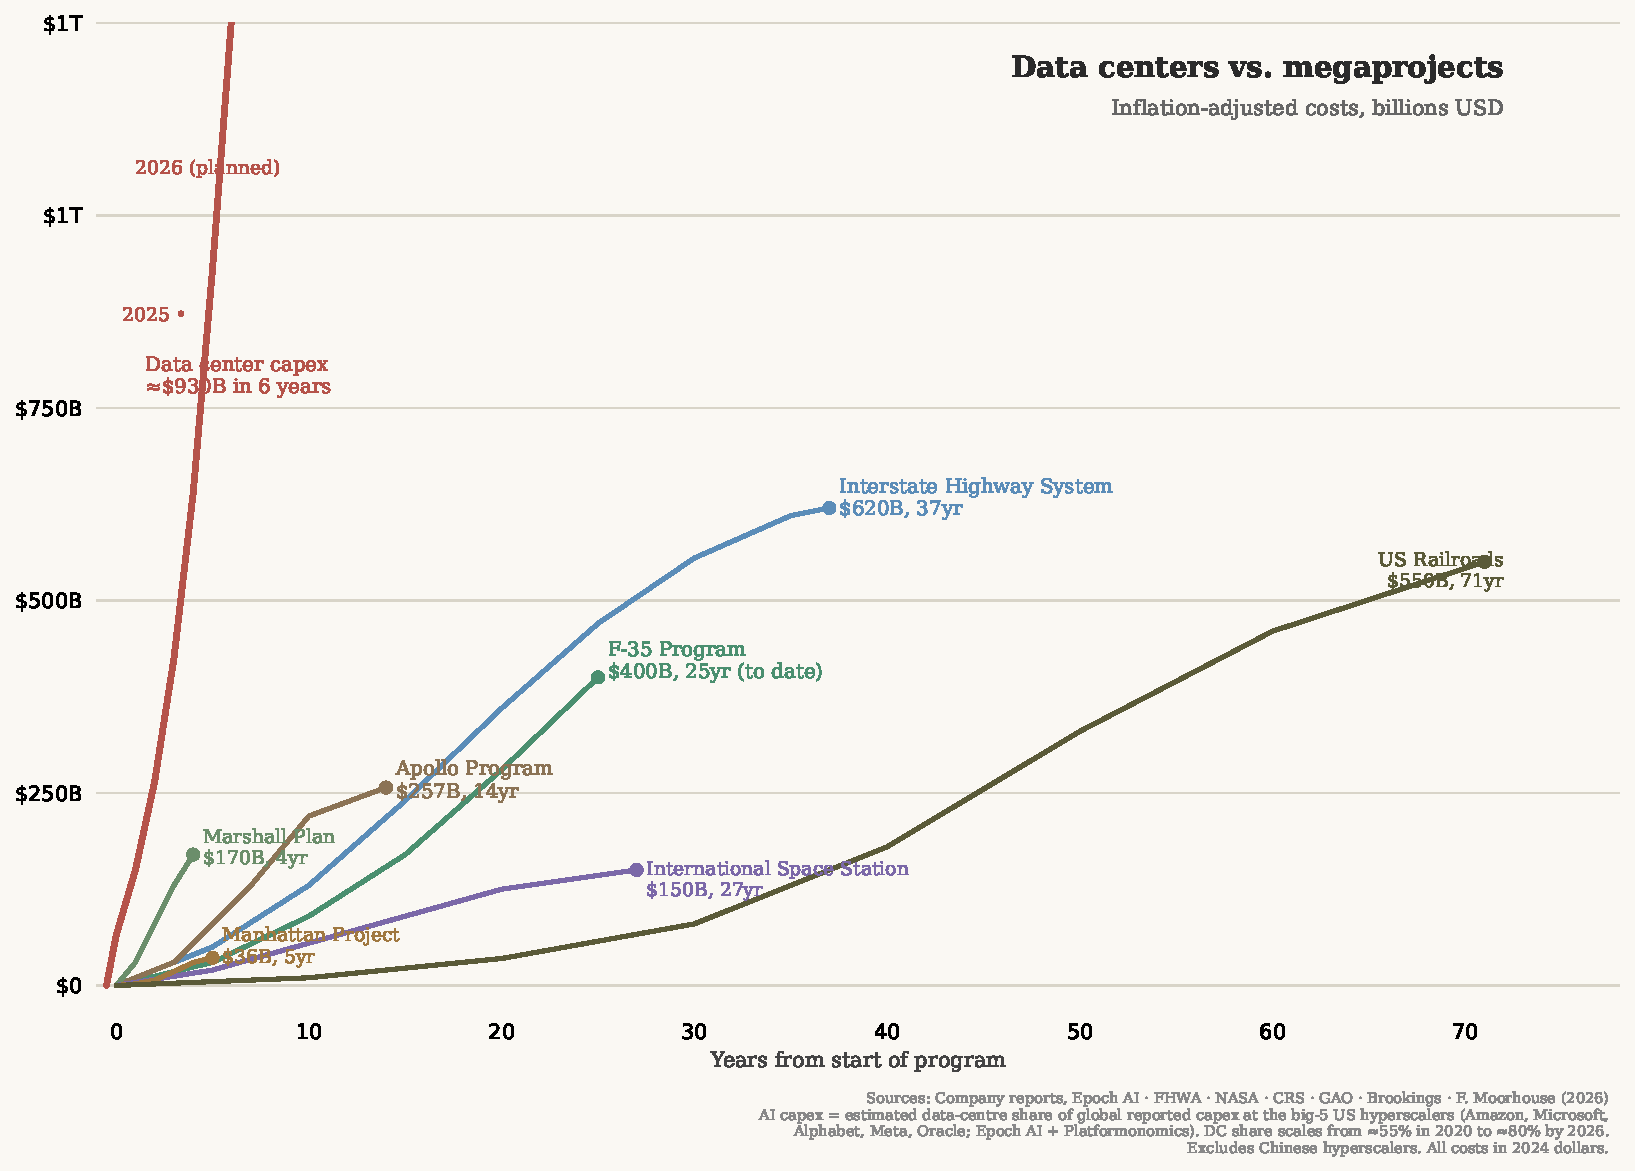
\includegraphics[width=\linewidth]{figures/megaprojects_capex}
\vspace{0.3em}
{\footnotesize\textit{Figure.} Cumulative data center capex (2019--2025, projected 2026) against
historical megaprojects, inflation-adjusted 2024 USD. Data: Epoch AI / Platformonomics;
FHWA; NASA; CRS; GAO; Brookings. Chart style after \citet{moorhouse2026megaprojects}.
All costs in 2024 dollars; Chinese hyperscalers excluded.}
\end{minipage}

\smallskip\noindent\rule{\linewidth}{0.3pt}\smallskip

\noindent\textbf{Why the comparison is powerful — and why it is also misleading.}\enspace
The chart circulates widely as evidence that data center investment has become the
defining infrastructure programme of the present moment, surpassing in speed and
aggregate cost anything the public sector has attempted since the Interstate Highway
System. As a rhetorical device it works: the visual comparison compresses the argument
into a single image.

As an analytical claim, however, the comparison conflates incommensurable categories.
\textit{First}, private recurring capital expenditure — distributed across thousands of
facilities, operators, and jurisdictions, repaid through commercial returns — is
structurally different from one-off public programmes underwritten by sovereign credit
and motivated by collective goods. The Apollo Programme produced the Moon landing and
was then wound down; data center capex is an indefinitely renewing operational
commitment whose cumulative figure grows by definition every year.
\textit{Second}, the comparison exploits the asymmetry of cumulation: summing six years
of annual private capex and setting it against the total lifetime cost of a 37-year
programme makes the former appear commensurately large, but the correct comparison is
the annual \textit{rate} of investment — at which point the Interstate Highway System
absorbed a larger share of US GDP for longer than the current data center build-out.
\textit{Third}, the data center capex figure rests on an opaque imputation methodology
(a DC share of hyperscaler capex scaling from $\approx$55\% to $\approx$80% across
the period) that is not independently verifiable and excludes Chinese hyperscalers
whose inclusion would substantially alter the comparison.
\textit{Fourth}, the selection of comparators does rhetorical work: there is no
equivalent chart for telecoms network buildout (1990--2000), rural electrification
(1935--1950), or the transatlantic cable system — all of which would likely produce
similar or larger figures on the same axes.

The chart is cited here not as authoritative evidence of scale but as a data point
about the \textit{genre of claim} being made about data centers in public discourse.
The fact that this particular comparison circulates as widely as it does — through
Epoch AI reports, policy briefs, and social media — is itself a finding: it indicates
that the governance and accountability frameworks for data center infrastructure are
being formed in an environment where the dominant reference points are wartime
mobilisation and Cold War programmes, not the regulatory regimes developed for
utilities, telecommunications, or land-use planning. The analogy shapes what
interventions appear plausible.

\end{tcolorbox}
\end{fullwidth}


A bibliometric audit of 4,757 publications with ``data center'' in the title on OpenAlex (2010--2025) makes the disciplinary gap visible in quantitative terms. The literature has grown by 372\% over fifteen years and organised itself into three structurally disconnected silos: technical efficiency (approximately 279 papers focused on cooling, power management, and hardware optimisation), environmental impact (approximately 114 papers, primarily on carbon footprint and energy sourcing), and socio-political dynamics (approximately 15 papers, including the rich ethnographic literature of \citet{vonderau2019storing} and \citet{holt2015vonderau}). Zero papers in this corpus engage the Multi-Level Perspective, Technological Innovation Systems, Strategic Niche Management, or sociotechnical regimes — the frameworks through which innovation scholars routinely analyse infrastructure transitions of comparable scale and consequence. The ethnographic work that does exist is invisible to this audience, and the innovation literature has not noticed the gap (\Cref{tab:silos}).

%% Inline tables — called from within body sections

%% ============================================================
%% Table 1 — Literature silos (called from sec:introduction)
%% ============================================================

\begin{table}[ht]
\centering
\caption{Three disconnected silos in the data center literature (OpenAlex, 2010--2025, $n = 4{,}757$).
         Representative works indicate the most-cited papers within each silo.
         The zero-paper row for innovation studies is the starting point of this research agenda.}
\label{tab:silos}
\setlength{\tabcolsep}{6pt}
\renewcommand{\arraystretch}{1.35}
\begin{tabularx}{\textwidth}{>{\bfseries}lXrX}
\toprule
\rowcolor{dcblue}
\textcolor{white}{\textbf{Silo}} &
\textcolor{white}{\textbf{Core focus}} &
\textcolor{white}{\textbf{$\approx n$}} &
\textcolor{white}{\textbf{Representative works}} \\
\midrule
Technical efficiency &
  Cooling infrastructure, power usage effectiveness (PUE), hardware lifecycle, workload scheduling, heat reuse &
  279 &
  \citet{dayarathna2015data}; Koomey (2011); \citet{masanet2020recalibrating} \\
\addlinespace[2pt]
\rowcolor{dcgray}
Environmental impact &
  Carbon footprint, scope 2 emissions, renewable energy PPAs, water withdrawal intensity &
  114 &
  \citet{iea2024electricity}; Jones (2018); Mytton \& Ashtine (2022) \\
\addlinespace[2pt]
Socio-political &
  Ethnography of infrastructure, planning disputes, cultural politics, local community impact &
  15 &
  \citet{blum2012tubes}; \citet{holt2015vonderau}; \citet{vonderau2019storing} \\
\addlinespace[4pt]
\rowcolor{dcaccent!12}
\textit{Innovation studies} &
  \textit{MLP, TIS, SNM, sociotechnical regimes, transition governance} &
  \textcolor{dcaccent}{\textbf{0}} &
  \textit{--- this paper ---} \\
\bottomrule
\end{tabularx}
\end{table}

%% ============================================================
%% Table 2 — Work packages (called from sec:introduction or sec:conceptual)
%% ============================================================

\begin{table}[ht]
\centering
\caption{The four work packages: CAS dimensions, data modalities, analytical outputs, and current implementation status.
         ``Seed'' denotes a pilot run against the three-operator facility index; ``design'' denotes a work package
         whose pipeline architecture is specified but not yet implemented.}
\label{tab:wps}
\setlength{\tabcolsep}{5.5pt}
\renewcommand{\arraystretch}{1.35}
\begin{tabularx}{\textwidth}{c>{\bfseries}lllXl}
\toprule
\rowcolor{dcblue}
\textcolor{white}{\textbf{WP}} &
\textcolor{white}{\textbf{CAS Dimension}} &
\textcolor{white}{\textbf{Primary method}} &
\textcolor{white}{\textbf{Data sources}} &
\textcolor{white}{\textbf{Key analytical output}} &
\textcolor{white}{\textbf{Status}} \\
\midrule
\textbf{1} & Conceptual &
  NLP / keyword scoring &
  Corporate websites; city Wikipedia &
  Environmental Claim Index (ECI); imaginary divergence score per operator--city pair &
  Seed run \\
\addlinespace[2pt]
\rowcolor{dcgray}
\textbf{2} & Conceptual &
  Computer vision (CLIP) &
  Sentinel-2 satellite imagery; corporate photography &
  Visual abstraction score; satellite--corporate imagery divergence &
  Design \\
\addlinespace[2pt]
\textbf{3} & Structural &
  Network analysis; spatial graph &
  OpenCorporates; REIT filings; Overture Maps (city2graph) &
  Ownership network + actor typology; urban embeddedness graph &
  Seed run \\
\addlinespace[2pt]
\rowcolor{dcgray}
\textbf{4} & Structural + Temporal &
  Topic modelling (BERTopic); event detection &
  News archives (GDELT/NewsAPI); planning records; social media &
  Signal-to-response lag; comparative contestation trajectory &
  Design \\
\bottomrule
\end{tabularx}
\end{table}

%% ============================================================
%% Table 3 — Virginia vs Amsterdam comparison
%% (called from sec:case)
%% ============================================================

\begin{table}[ht]
\centering
\caption{Comparative dimensions: Northern Virginia (Loudoun County) and Amsterdam.
         Both markets exhibit high community contestation intensity.
         The decisive variable differentiating regime responses is not signal strength
         but the structural architecture of the receiving system.
         ECI figures from WP1 seed run (April 2026); urban embeddedness from WP3 seed run (April 2026).}
\label{tab:comparison}
\setlength{\tabcolsep}{6pt}
\renewcommand{\arraystretch}{1.4}
\begin{tabularx}{\textwidth}{>{\bfseries\small}lXX}
\toprule
\rowcolor{dcblue}
\textcolor{white}{\textbf{Dimension}} &
\textcolor{white}{\textbf{Northern Virginia (Loudoun County)}} &
\textcolor{white}{\textbf{Amsterdam}} \\
\midrule
Operator type &
  Hyperscale (AWS, Microsoft, Google, Meta) + colocation (Equinix, Digital Realty, CyrusOne) &
  Hyperscale + colocation (Equinix AMS campus) + cooperative exchange (AMS-IX) \\
\addlinespace[2pt]
\rowcolor{dcgray}
Ownership structure &
  REIT-dominated; beneficial ownership dispersed across global pension funds and retail investors &
  Mixed; operator-owned campuses, cooperative exchange, concentrated sovereign wealth fund positions \\
\addlinespace[2pt]
Governance counterparty &
  None identifiable; operating entity legally separated from asset-owning REIT &
  Municipality (Amsterdam) with legal planning competence; named operator counterparties \\
\addlinespace[2pt]
\rowcolor{dcgray}
Urban embeddedness (2~km) &
  36 power-infra nodes; \textbf{1} residential zone; \textbf{0} adjacency edges~--- exurban spatial segregation &
  2 power nodes; \textbf{61} residential zones; \textbf{16} adjacency edges~--- embedded in urban fabric \\
\addlinespace[2pt]
Territorial imaginary &
  Opportunity framing; placeless; ECI divergence \textbf{165.7} (corp 167.1 vs.\ wiki 1.4) &
  Contested, partially negotiated; lower ECI divergence; regulatory vocabulary absorbed \\
\addlinespace[2pt]
\rowcolor{dcgray}
Visual regime &
  High abstraction; hyperscale anonymity; near-zero facility-level disclosure &
  Lower abstraction; higher regulatory disclosure requirements; urban-context imagery \\
\addlinespace[2pt]
Contestation intensity &
  High; community campaigns, planning hearing backlogs, state-level water studies &
  High; sustained municipal and civic mobilisation, media coverage, moratorium petitions \\
\addlinespace[2pt]
\rowcolor{dcgray}
Regime response &
  None; no moratorium; operator-accommodating state permitting environment &
  Moratorium declared 2019; enforced 2019--2022; lifted under differentiated energy/water criteria \\
\addlinespace[4pt]
\rowcolor{dclightyellow}
\multicolumn{1}{>{\bfseries\small\color{dcaccent}}l}{Explanatory variable} &
  \textcolor{dcaccent}{Dispersed ownership and absent governance counterparty insulate regime from community pressure} &
  \textcolor{dcblue}{Concentrated, accountable ownership + empowered municipal authority enable binding negotiation} \\
\bottomrule
\end{tabularx}
\end{table}


This paper makes three contributions in response. First, it proposes \textit{datacentering} as a conceptual reframing — a gerund that foregrounds the active, contested, ongoing process of assembling digital infrastructure over time, rather than treating data centers as fixed technical objects amenable to efficiency optimisation. Second, it develops a multimodal research agenda structured around the conceptual and structural dimensions of these assemblages, drawing on complex adaptive systems (CAS) thinking \citep{phillips2019complex} as a sensemaking lens for understanding phenomena that are constituted by multi-actor constellations — corporations, financial investors, planning authorities, municipal governments, communities, and nonhuman actors including power grids, aquifers, and fibre networks — whose interactions produce emergent, nonlinear outcomes no single actor controls. Third, it argues that the CAS-like character of these phenomena is itself the reason why no single researcher or team can build the cartography required: the geography is too large, the data too distributed, and the opacity too deliberate. We therefore accompany this paper with an open research infrastructure — a community-maintained facility index, shared analytical pipelines, and open data — as a theoretically motivated response to the complexity of the object, and as an invitation to collective knowledge production.

The paper proceeds as follows. \Cref{sec:background} reviews the relevant literature and introduces the concept of datacentering and the CAS sensemaking lens. \Cref{sec:conceptual} develops the conceptual dimension of the research agenda, addressing how actors construct the imaginaries and territorial claims that make data center infrastructure legible or illegible. \Cref{sec:structural} addresses the structural dimension, mapping the ownership hierarchies and actor constellations — including the urban and municipal actors that the city2graph framework \citep{city2graph} makes tractable — through which governance capacity (or its absence) is constituted. \Cref{sec:temporal} addresses the temporal dimension, examining how contestation signals unfold over time and what determines whether regime actors respond. \Cref{sec:case} illustrates the framework through a comparison of Northern Virginia and Amsterdam, two markets with equivalent contestation intensity but structurally different governance responses. \Cref{sec:discussion} draws out the theoretical implications and positions the open cartography as a research programme. \Cref{sec:conclusion} closes with the invitation to build it together.
